\colorlet{other}{brown}
\colorlet{philo}{other}
\colorlet{lingu}{other}
\colorlet{neuro}{other}
\colorlet{psycho}{other}
\colorlet{bscarb}{other}


\DTLsetpiesegmentcolor{1}{kogni}
\DTLsetpiesegmentcolor{2}{info}
\DTLsetpiesegmentcolor{3}{mathe}
\DTLsetpiesegmentcolor{4}{other}
\DTLsetpiesegmentcolor{5}{sq}

\begin{Huge}
    Kognitionswissenschaft
\end{Huge}

\begin{exampleblock}{\textcolor{white}{Was ist der Studiengang?}}
    Ein sehr interdisziplinärer Studiengang, der einzelne Aspekte der Informatik, (Neuro-)Biologie, Linguistik, Philosophie und Psychologie miteinander verbindet, bzw. auch einzeln behandelt. Alle Fragen, die dem Denken gewidmet sind, finden hier ihren Platz und werden mithilfe der verschiedenen Sichtweisen der unterschiedlichen Disziplinen versucht zu beantworten. Ein Schwerpunktfach gibt es nicht. Danach kann das Studium mit einem Master (4 Semester Regelstudienzeit) weitergeführt werden.
\end{exampleblock}

\begin{block}{Welcher Teil macht wie viel im Studium aus?}
    \begin{figure}[h!]
        \begin{minipage}{\linewidth}
            \centering
            \DTLloaddb{LPverteilungKogni}{inhalte/kogni.csv}
            \tikzstyle{every node}=[text width={},minimum height=0pt]
            \DTLpiechart{
                variable=\lp,
                innerlabel={\parbox{40pt}{\centering\color{white} \bereich}},
                innerratio=0.25,
                radius=70pt,
                rotateinner}{LPverteilungKogni}{\bereich=Bereich,\lp=LP}
        \end{minipage}
        \vspace{-20pt}
        \caption{Verteilung der Themenbereiche über das komplette Studium}
    \end{figure}
\end{block}

\begin{block}{Was macht man in welchem Semester?}
    \begin{figure}[h!]
        % 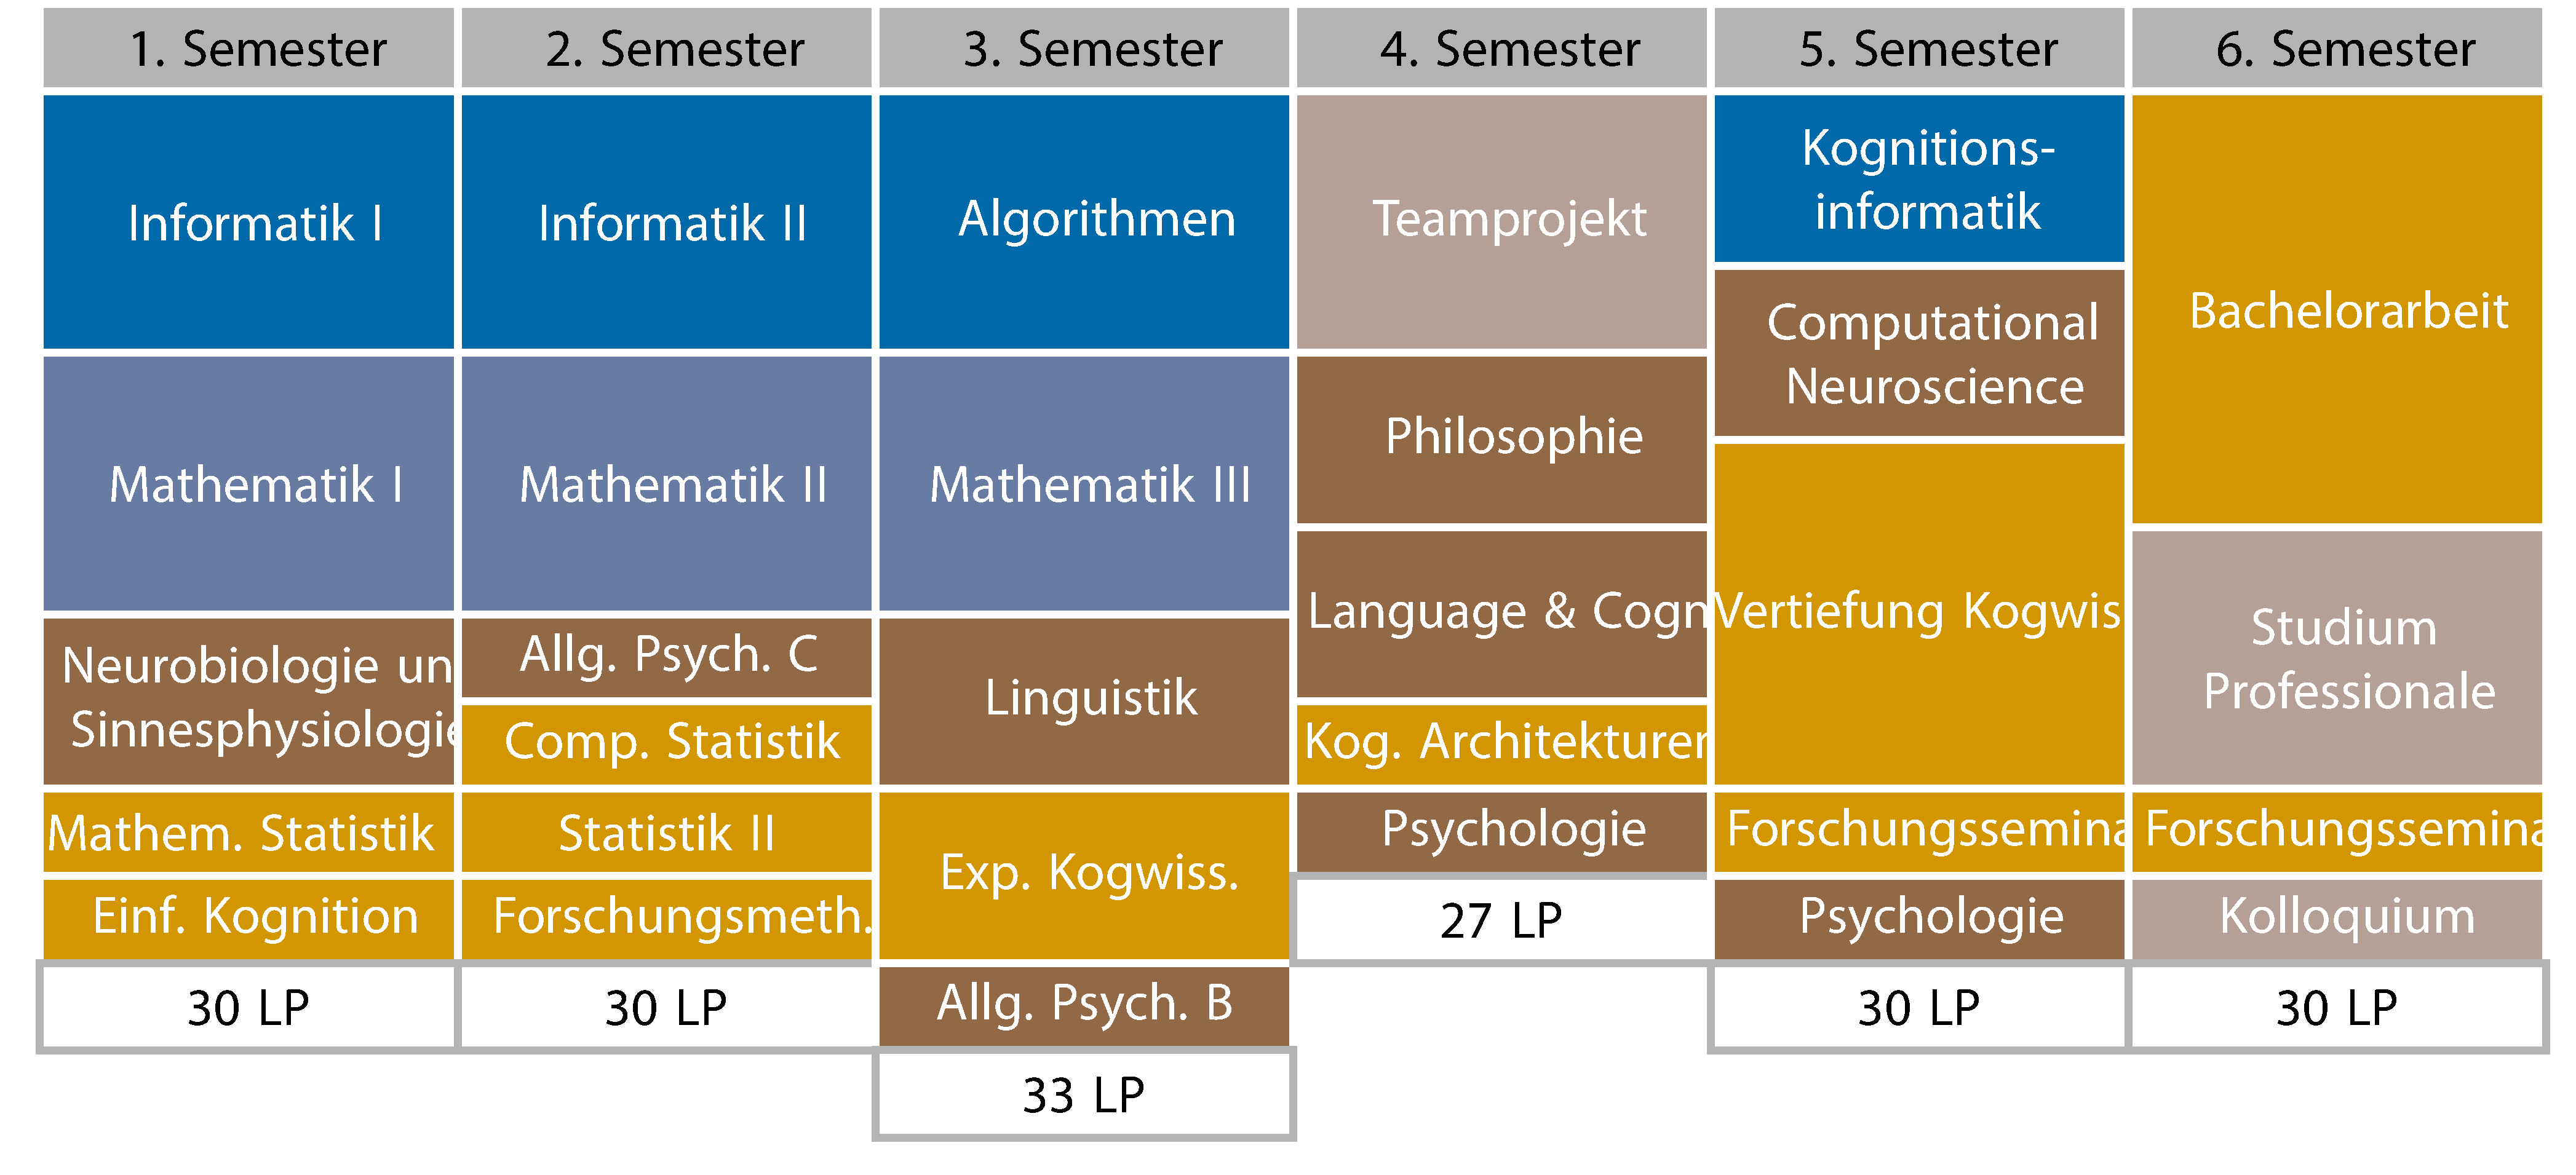
\includegraphics[width=\textwidth]{charts/kognitionswissenschaft_StudienplanabWS18.pdf}
        \resizebox{\linewidth}{!}{
        \begin{minipage}{\textwidth}
            \small
            \begin{tikzpicture}
                \begin{scope}[start chain=going below,node distance=\nodedistancecorrection]
                    \semester{1}
                    \veranstaltung{9}{In\-for\-ma\-tik~I}{info}
                    \veranstaltung{9}{Mathe\-matik~I}{mathe}        
                    \veranstaltung{6}{Neuro\-bio\-logie und Sinnes\-physio\-logie}{neuro}
                    \veranstaltung{3}{Mathem. Statistik I}{kogni}
                    \veranstaltung{3}{Einf.\ Kognition}{kogni}
                    \SumLP{30}
                \end{scope}
                \begin{scope}[xshift=1\lpwidth,start chain=going below,node distance=\nodedistancecorrection]
                    \semester{2}
                    \veranstaltung{9}{In\-for\-ma\-tik~II}{info}
                    \veranstaltung{9}{Mathe\-matik~II}{mathe}
                    \veranstaltung{3}{Allg. Psych. C}{psycho}
                    \veranstaltung{3}{Comp. Statistik}{kogni}
                    \veranstaltung{3}{Statistik II}{kogni}
                    \veranstaltung{3}{Forschungsmeth.}{kogni}
                    \SumLP{30}
                \end{scope}
                \begin{scope}[xshift=2\lpwidth,start chain=going below,node distance=\nodedistancecorrection]
                    \semester{3}
                    \veranstaltung{9}{Al\-go\-rith\-men}{info}
                    \veranstaltung{9}{Mathe\-matik~III}{mathe}
                    \veranstaltung{6}{Linguistik}{lingu}
                    \veranstaltung{6}{Exp. Kogwiss.}{kogni}
                    \veranstaltung{3}{Allg. Psych. B}{psycho}
                    \SumLP{33}
                \end{scope}
                \begin{scope}[xshift=3\lpwidth,start chain=going below,node distance=\nodedistancecorrection]
                    \semester{4}     
                    \veranstaltung{9}{Team\-projekt}{sq}
                    \veranstaltung{6}{Philosophie}{philo}
                    \veranstaltung{6}{Language \& Cogn.}{lingu}
                    \veranstaltung{3}{Kog. Architekturen}{kogni}
                    \veranstaltung{3}{Psychologie}{psycho}
                    \SumLP{27}
                \end{scope}
                \begin{scope}[xshift=4\lpwidth,start chain=going below,node distance=\nodedistancecorrection]
                    \semester{5}
                    \veranstaltung{6}{Kognitions\-informatik}{info}
                    \veranstaltung{6}{Computational Neuroscience}{neuro}
                    \veranstaltung{12}{Vertiefung Kogwiss.}{kogni}
                    \veranstaltung{3}{Forschungsseminar}{kogni}
                    \veranstaltung{3}{Psychologie}{psycho}
                    \SumLP{30}
                \end{scope}
                \begin{scope}[xshift=5\lpwidth,start chain=going below,node distance=\nodedistancecorrection]
                    \semester{6}
                    \veranstaltung{15}{Bachelor\-arbeit}{kogni}
                    \veranstaltung{9}{Studium Professionale}{sq}
                    \veranstaltung{3}{Forschungsseminar}{kogni}
                    \veranstaltung{3}{Kolloquium}{sq}
                    \SumLP{30}
                \end{scope}
            \end{tikzpicture}
        \end{minipage}}        
    \end{figure}

    Das 1. Semester ist nach Plan ein Wintersemester, der Studienbeginn ist hier auch nur zum Wintersemester möglich. 
    Dieser Verlauf ist lediglich ein Vorschlag und kein bindender Studienplan. Es empfiehlt sich jedoch, den Plan einzuhalten, wenn man in Regelstudienzeit studieren möchte.
\end{block}

\vfill
\begin{flushright}
    
\includegraphics[width=0.4\textwidth]{images/fsilogo.pdf}
\end{flushright}